\chapter{Parts}
The following is a comprehensive parts list and should be used as both documentation of the individual parts, but it also serves as a printing and buying reference. We do not favor or represent anybody but ourselves, so prices and links to reseller are only meant as a guideline. The design being open-source, you can easily swap out parts and adapt the design to fit your requirements.


\addthumb{\LARGE\quad Parts}{\LARGE\ding{52}}{white}{titlepagecolor!55}

\section{3D printed parts}

All 3D printed parts have been designed using SolidWorks by Dassault Systems and printed on PLA using Ultimaker Original 3D Printers and Bq Witbox 3D Printers, where the Witbox was used for the larger parts that physically could not fit the Ultimaker. Unless otherwise stated, parts were printed using a Layer height of 0.2mm, Shell thickness of 0.8mm, Bottom/Top thickness of 1.6mm and a varying Fill density between 20-50\%. Settings may vary depending on your specific printer setup.

\subsection{Yaw joint ($\times1$)}

\begin{wrapfigure}{r}{0.25\textwidth}
    \vspace{-1.5cm}
    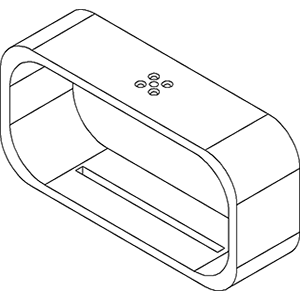
\includegraphics[width=0.25\textwidth]{PrintedParts/yaw_joint.PNG}
\end{wrapfigure}

The yaw joint acts as a joint between the grip arm and the top U bracket. It is designed so the weight of the gimbal compresses the yaw motor instead of pulling it apart.\\

\raisebox{-0.2cm}{\hspace{-1.5cm}\Huge\Info}\normalsize \quad Print laying down and with a vertical O-profile. No support material.


\subsection{Joystick case ($\times1$)}

\begin{wrapfigure}{r}{0.25\textwidth}
    \vspace{-1.5cm}
    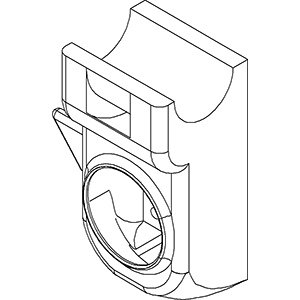
\includegraphics[width=0.25\textwidth]{PrintedParts/joystick_case.PNG}
\end{wrapfigure}

The joystick case is designed to contain the joystick and fit the construction.\\

\raisebox{-0.2cm}{\hspace{-1.5cm}\Huge\Info}\normalsize \quad Print in two separate parts with the flattest side facing down. Support material touching buildplate.\\\\\\


\subsection{Grip arm left ($\times1$) and right ($\times1$)}

\begin{wrapfigure}{r}{0.25\textwidth}
    \vspace{-1.65cm}
    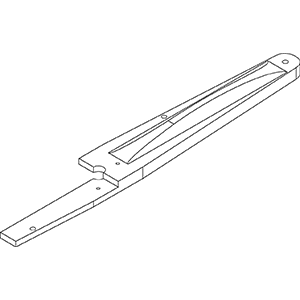
\includegraphics[width=0.25\textwidth]{PrintedParts/grip_arm_right.PNG}
\end{wrapfigure}

The grip arm attaches to the yaw joint and is divided in two parts.\\

\raisebox{-0.2cm}{\hspace{-1.5cm}\Huge\Info}\normalsize \quad Print in two separate parts with the flattest side facing down. Support material touching buildplate.


\subsection{Handle ($\times3$)}	

\begin{wrapfigure}{r}{0.25\textwidth}
    \vspace{-2cm}
    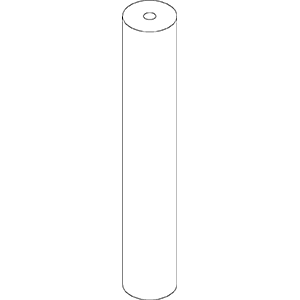
\includegraphics[width=0.25\textwidth]{PrintedParts/handle.PNG}
\end{wrapfigure}

Two handles attach to the grip arm to allow holding the gimbal with two hands. 

A third handle can be attached to the optional one-hand grip arm to allow for one handed handling.\\

\raisebox{-0.2cm}{\hspace{-1.5cm}\Huge\Info}\normalsize \quad Print upright, to make for a good screw hole in the middle. No support material.


\subsection{Bracket L $\times3$}
\begin{wrapfigure}{r}{0.25\textwidth}
    \vspace{-1cm}
    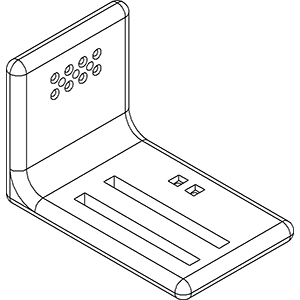
\includegraphics[width=0.25\textwidth]{PrintedParts/bracket_L.PNG}
\end{wrapfigure}

The L bracket is the main mounting point for the camera. 

As such, it needs to be especially rigid, which is why it is the most robustly designed part. 

The L bracket is attached to the bottom U bracket through the roll motor.\\

\raisebox{-0.2cm}{\hspace{-1.5cm}\Huge\Info}\normalsize \quad Print on its side with a vertical L-profile. No support material.


\subsection{Bracket U Bottom $\times3$}

\begin{wrapfigure}{r}{0.25\textwidth}
    \vspace{-1.5cm}
    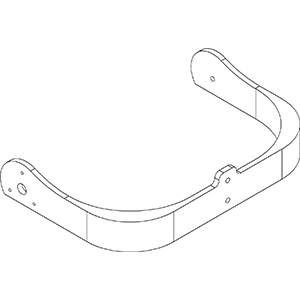
\includegraphics[width=0.25\textwidth]{PrintedParts/bracket_U_top.PNG}
\end{wrapfigure}

The bottom U bracket is attached to the top U bracket through the pitch motor. On its back side, the main electronics board can be mounted.\\

\raisebox{-0.2cm}{\hspace{-1.5cm}\Huge\Info}\normalsize \quad Print with a vertical U profile. No support material.


\subsection{Bracket U Top $\times3$}

\begin{wrapfigure}{r}{0.25\textwidth}
    \vspace{-3cm}
    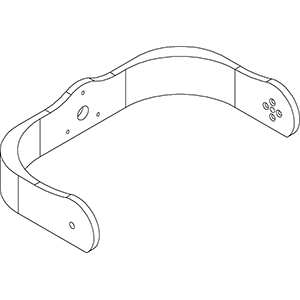
\includegraphics[width=0.25\textwidth]{PrintedParts/bracket_U_bottom.PNG}
\end{wrapfigure}

The top U bracket is attached to the yaw joint through the yaw motor.\\

\raisebox{-0.2cm}{\hspace{-1.5cm}\Huge\Info}\normalsize \quad Print with a vertical U profile. No support material.


\subsection{Grip arm one-hand $\times3$}

\begin{wrapfigure}{r}{0.25\textwidth}
    \vspace{-3cm}
    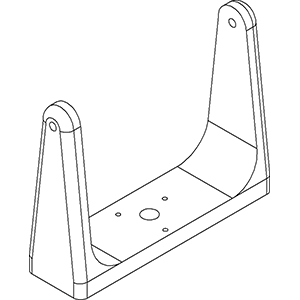
\includegraphics[width=0.25\textwidth]{PrintedParts/grip_arm_onehand.PNG}
\end{wrapfigure}

The one-hand grip arm is mounted between the yaw joint and the grip arm and allows for one-handed operation.\\

\raisebox{-0.2cm}{\hspace{-1.5cm}\Huge\Info}\normalsize \quad
Print either pointing upwards with no support material or horizontally positioned to make for at stronger part with support material touching buildplate.


\subsection{Case for simpleBCG 8-bit main board ($\times3$)}

\begin{wrapfigure}{r}{0.25\textwidth}
    \vspace{-1.5cm}
    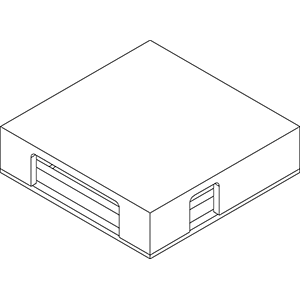
\includegraphics[width=0.25\textwidth]{PrintedParts/case_main_assembly.PNG}
\end{wrapfigure}

The case is used to mount and secure the AlexMos simpleBCG 8-bit controller mainboard. This design is easily reconfigured in SolidWorks to match other board designs.\\

\raisebox{-0.2cm}{\hspace{-1.5cm}\Huge\Info}\normalsize \quad
Print bottom and top parts separately lying flat. No support material.


\subsection{Case for simpleBCG yaw extension board ($\times3$)}

\begin{wrapfigure}{r}{0.25\textwidth}
    \vspace{-1.5cm}
    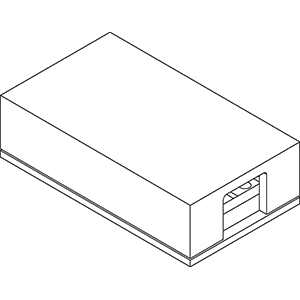
\includegraphics[width=0.25\textwidth]{PrintedParts/case_yaw_assembly.PNG}
\end{wrapfigure}

The case is used to mount and secure the AlexMos SimpleBCG yaw extension board. 

This design is easily reconfigured in SolidWorks to match other board designs.\\

\raisebox{-0.2cm}{\hspace{-1.5cm}\Huge\Info}\normalsize \quad
Print bottom and top parts seperately laying flat. No support material.\\


\section{Third party electronics}
The following third party parts are required to stabilize the system. The specific chosen parts are guidelines and can be replaced with similar parts.

\subsection{BaseCam SimpleBGC 8-bit Set ($\times1$)}

\begin{wrapfigure}{r}{0.25\textwidth}
    \vspace{-1.5cm}
    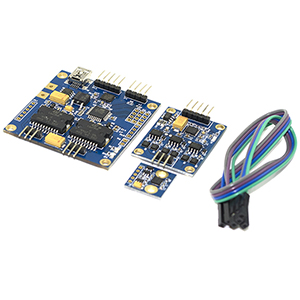
\includegraphics[width=0.25\textwidth]{ThirdParts/SimpleBGC.jpg}
\end{wrapfigure}

Our choice of electronics is the BaseCam SimpleBCG 8-bit.

Electronics are required to control the three brushless motors. An IMU (inertial measurement unit) sensor provides the main board with feedback on the camera’s inertial state. Specifically it contains a gyroscope, accelerometer and magnetometer.

For this implementation, the BaseCam SimpleBGC 8-bit controller set \footnote{\url{http://www.basecamelectronics.com/simplebgc/}} is used, consisting of a main board, a yaw extension board and an Inertial Measurement Unit (IMU).\\\\

\raisebox{-0.2cm}{\hspace{-1.5cm}\Huge\Info}\normalsize \quad Practically, the BaseCam SimpleBGC 32-bit, STorM32 or any other electronics for controlling the motors can be used, but the main and yaw cases need to be adapted to fit the board’s specifications.\\

\subsection{Brushless gimbal motors ($\times3$)}

\begin{wrapfigure}{r}{0.25\textwidth}
    \vspace{-1.5cm}
    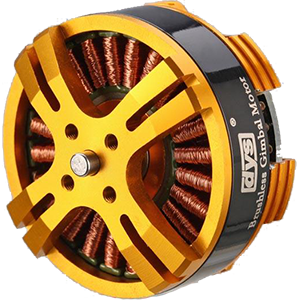
\includegraphics[width=0.25\textwidth]{ThirdParts/Motor.png}
\end{wrapfigure}

The motors used are type BGM4108 brushless gimbal motors by WST \footnote{\url{http://www.ebay.com/itm/WST-Brushless-Gimbal-Motor-BGM4108-130T-for-Camera-Mount-FPV-PTZ-/281343734210?pt=LH_DefaultDomain_0&hash=item418164b1c2}}. Other manufacturers of the BGM4108 include RCTimer and DYS. For the smoothest operation, select motors with many poles ($\geq14$) and many turns ($\geq100$).\\

\raisebox{-0.2cm}{\hspace{-1.5cm}\Huge\Info}\normalsize \quad Practically, any suitable motor can be used, but screw holes need to be adapted to fit the motor’s specifications. Also, the motors should have a sufficient number of poles for fine adjustments.\\


\subsection{Battery ($\times1$)}

\begin{wrapfigure}{r}{0.25\textwidth}
    \vspace{-1.5cm}
    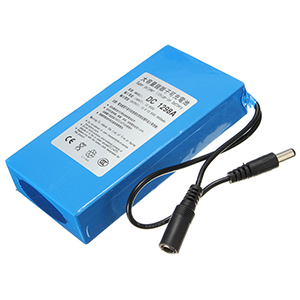
\includegraphics[width=0.25\textwidth]{ThirdParts/Battery.PNG}
\end{wrapfigure}

A 12V $\sim$4000mAh Lithium Polymer (LiPo) battery was used to power the motors and electronics. \footnote{\url{http://www.banggood.com/DC12V-9800mAh-Super-Rechargeable-Protable-Lithium-Battery-EU-Plug-p-963254.html}} This is sufficient to power \textbf{\textsf{OpenSAM}} for more than 3 hours.\\

\raisebox{-0.2cm}{\hspace{-1.5cm}\Huge\Info}\normalsize \quad Practically, any 8-18V battery can be used, but care should be taken on the current it can deliver and the capacity it stores. Size and weight may also be significant factors. Current consumption is estimated to peak at 2A.\\

\raisebox{-0.2cm}{\hspace{-1.5cm}\Huge\Radioactivity}\normalsize \quad Make sure to connect the battery with the correct polarity!\\


\subsection{Joystick with button ($\times1$)}

\begin{wrapfigure}{r}{0.25\textwidth}
    \vspace{0.1cm}
    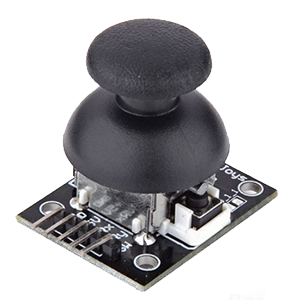
\includegraphics[width=0.25\textwidth]{ThirdParts/Joystick.PNG}
\end{wrapfigure}

The joystick allows user input to the controller to adjust the angles of the camera. It also contains a button which we choose to use to calibrate the IMU, stop the motors and reset the controller.
For a guide on how to setup the Arduino compatible PS2 joystick we used \footnote{\url{http://www.banggood.com/PS2-Game-Joystick-Module-For-Arduino-p-76465.html}} see the configuration chapter of this manual.\\

\raisebox{-0.2cm}{\hspace{-1.5cm}\Huge\Info}\normalsize \quad Practically any joystick can be used, but compatibility to the electronics need to be insured and the joystick case needs to be adapted to fit the joystick’s specifications. 


\section{Generic parts}
The used brushless gimbal motors and electronics for this project included cables for connecting these and they are thus not listed here. The motors also came with screws inclusive, these were however not long enough for this application.

\subsection{M2.5 Screws ($\times9$)}

\begin{wrapfigure}{r}{0.25\textwidth}
    \vspace{-1.5cm}
    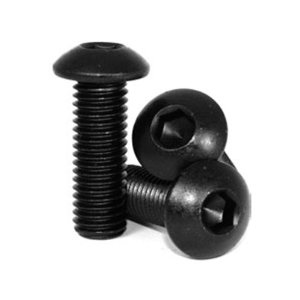
\includegraphics[width=0.25\textwidth]{GenericParts/M25Screws.jpg}
\end{wrapfigure}

M2.5 screws are needed to attach the fixed part of gimbal motors to the system.

6x15mm and 3x25mm M2.5 screws are used if using the optional one-handed grip arm.

9x15mm M2.5 screws are used if not using the one-handed grip arm.


\subsection{M3 Screws ($\times14$) and M3 nuts ($\times2$)}

\begin{wrapfigure}{r}{0.25\textwidth}
    \vspace{-1.5cm}
    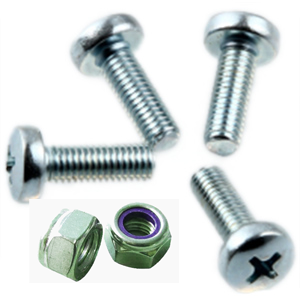
\includegraphics[width=0.25\textwidth]{GenericParts/M3ScrewsLocknuts.png}
\end{wrapfigure}

12x15mm M3 screws are used for attaching the moving part of the motors to the system.

2x15mm M3 screws combined with 2xM3 nuts are used to attach the left and the right parts of the grip arm.\\

\raisebox{-0.2cm}{\hspace{-1.5cm}\Huge\Info}\normalsize \quad For the nuts, it is recommended to use locking nuts (locknuts).


\subsection{M4 Screws ($\times3$) and M4 nuts ($\times3$)}

\begin{wrapfigure}{r}{0.25\textwidth}
    \vspace{-1.5cm}
    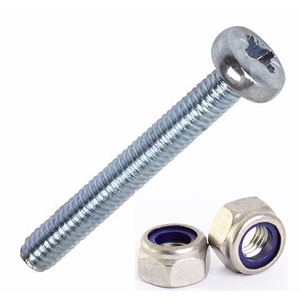
\includegraphics[width=0.25\textwidth]{GenericParts/M4ScrewsLocknuts.png}
\end{wrapfigure}

1x20mm M4 screws (or longer) and 1xM4 nut (loose) are used for attaching the top U bracket to the bottom U bracket on the side opposing the pitch motor.

2x20mm M4 screws (or longer) and 2xM4 nuts are used for attaching the grip arm to the top U bracket.\\

\raisebox{-0.2cm}{\hspace{-1.5cm}\Huge\Info}\normalsize \quad For the nuts, it is recommended to use locking nuts (locknuts).


\subsection{Wood Screws ($\times2+\times2$)}

\begin{wrapfigure}{r}{0.25\textwidth}
    \vspace{-1.5cm}
    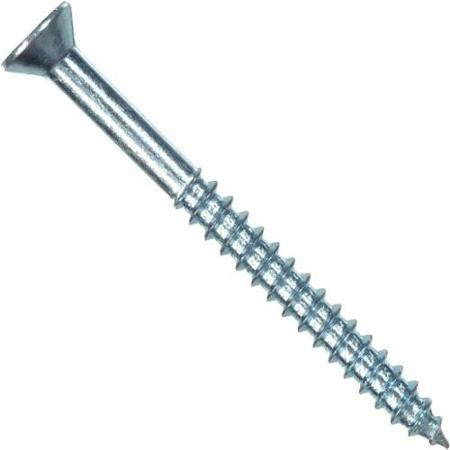
\includegraphics[width=0.2\textwidth]{GenericParts/WoodScrew.jpg}
\end{wrapfigure}

The wood screws screw into the handles. Their length is stated approximately.

2x80mm with a diameter of ca. 4mm are used to fixate the outer handles.

2x40mm also with a diameter of ca. 4mm are used for the optional one-handed grip arm.

\begin{wrapfigure}{r}{0.25\textwidth}
    \vspace{-1.5cm}
    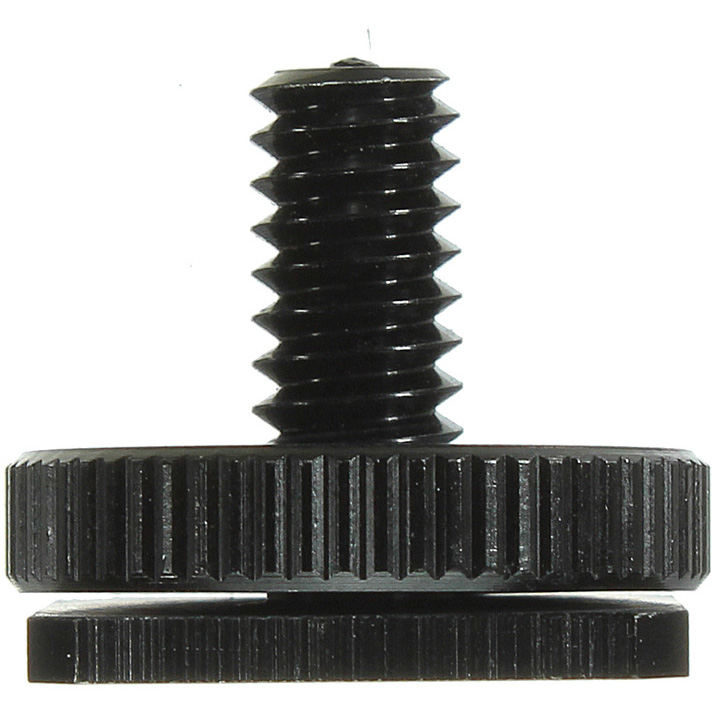
\includegraphics[width=0.2\textwidth]{GenericParts/Thumbscrew.JPG}
\end{wrapfigure}

\subsection{Camera mounting screw ($\times1$)}

The standard camera mounting screw thread size is per ISO 1222:2010 1/4-20 UNC. Optimally use a thumbscrew. Also, ensure sufficient length of the screw, at least 30mm.


\subsection{Reattachable fasteners (ca. 40 cm)}

\begin{wrapfigure}{r}{0.25\textwidth}
    \vspace{-1.5cm}
    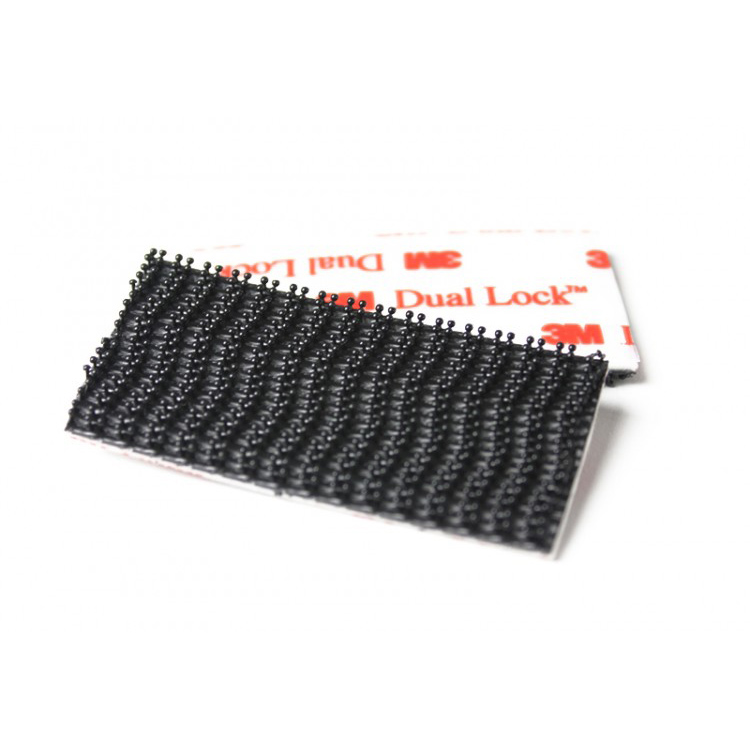
\includegraphics[width=0.2\textwidth]{GenericParts/Dual-lock.jpg}
\end{wrapfigure}

To mount the battery and electronic boxes to the system, we used reattachable “Dual lock” fasteners for easy attachment and removal of the parts. Approximately 40cm were used. \footnote{\url{http://solutions.3m.com/wps/portal/3M/en_US/Adhesives/Tapes/Brands/Dual-Lock-Reclosable-Fasteners/}}\\
Any adhesive could also be used, but this would compromise on the convenience.


\subsection{Cable extensions (optional)}

\begin{wrapfigure}{r}{0.25\textwidth}
    \vspace{-1.5cm}
    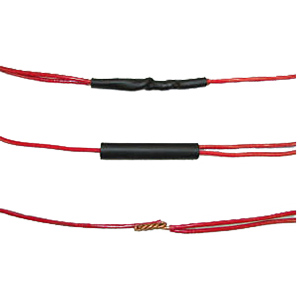
\includegraphics[width=0.2\textwidth]{GenericParts/Cable-extension.jpg}
\end{wrapfigure}

The provided cables for the electronics was a little bit short for optimal cable management and were extended using generic cables, a soldering iron and heat shrink tubes.

